% This is samplepaper.tex, a sample chapter demonstrating the
% LLNCS macro package for Springer Computer Science proceedings;
% Version 2.20 of 2017/10/04
%
\documentclass[runningheads]{llncs}
%
\usepackage{graphicx}

%%%%ДОБАВИЛ ДЛЯ РУССКОГО ТЕКСТА
%\usepackage[utf8x]{inputenc}
%\usepackage[english,russian]{babel}
%\usepackage{cmap}
%%%%


% If you use the hyperref package, please uncomment the following line
% to display URLs in blue roman font according to Springer's eBook style:
% \renewcommand\UrlFont{\color{blue}\rmfamily}

\begin{document}
%
\title{Adaptive global optimization based on nested dimensionality 
reduction\thanks{This study was supported by the Russian Science Foundation, 
project No.\,16-11-10150.}}
%
\titlerunning{Adaptive global optimization}
% If the paper title is too long for the running head, you can set 
% an abbreviated paper title here
%
\author{Konstantin Barkalov %\orcidID{0000-0001-5273-2471}  
\and Ilya Lebedev %\orcidID{0000-0002-8736-0652}
}
%
\authorrunning{K. Barkalov, I. Lebedev}
% First names are abbreviated in the running head.
% If there are more than two authors, 'et al.' is used.
%
\institute{Lobachevsky State University of Nizhni Novgorod, Nizhni Novgorod, 
Russia \email{konstantin.barkalov@itmm.unn.ru}}
%
\maketitle              % typeset the header of the contribution
%
\begin{abstract}

In the present paper, the multidimensional multiextremal optimization 
problems and the numerical methods for solving these ones are considered. A 
general assumption only is made on the objective function that this one 
satisfies the Lipschitz condition with the Lipschitz constant not known 
a priori. The problems of this type are frequent in the applications. 
Two approaches to the dimensionality reduction for the multidimensional 
optimization problems were considered. The first one uses the Peano-type 
space-filling curves mapping a one-dimensional interval onto a multidimensional 
domain. The second one is based on the nested optimization scheme, which 
reduces a multi-dimensional problem to a family of the one-dimensional 
subproblems. A generalized scheme combining these two approaches has been 
proposed. In this novel scheme, solving a multidimensional problem is 
reduced to solving a family of problems of lower dimensionality, in 
which the space-filling curves are used. An adaptive algorithm, in which all 
arising subproblems are solved simultaneously has been implemented. The 
numerical experiments on several hundred test problems have been carried out 
confirming the efficiency of the proposed generalized scheme.

\keywords{Global optimization \and Multiextremal functions \and 
Dimensionality reduction \and Peano curve \and Nested optimization \and 
Numerical methods.}
\end{abstract}
%
%
%
\section{Introduction}
This paper considers ``black-box'' global optimization problems of the 
following form:
\begin{eqnarray}\label{main_problem}
& \varphi(y^\ast)=\min{\left\{\varphi(y):y\in D\right\}},\\
& D=\left\{y\in R^N: a_i\leq y_i \leq b_i, 1\leq i \leq N\right\}. \nonumber
\end{eqnarray}
The objective function is assumed to satisfy the Lipschitz condition 
\[
\left|\varphi(y')-\varphi(y'')\right|\leq L\left\|y'-y''\right\|,\; y',y'' \in
 D,\; 0<L<\infty,
\]
with the constant $L$ unknown a priori.

The multistart scheme is a well known method for solving the multiextremal problems.
In such schemes, a grid is seeded in the search domain, the points of which are used as the starting ones for the search of 
the extrema by some local method, and then the lowest of the found extrema is chosen. 
The choice of the starting points performed, as a rule, on the basis of the Monte Carlo method is a special problem within 
this approach \cite{Zhigljavsky2008}. 
The approach is well applicable for the problems with a small number of local minima having a vide field of application, 
but for the problems with essential multiextremality its efficiency falls drastically. 

At present, the genetic algorithms one way or another based on the random search concept are used widely for solving the 
global optimization problems (see, for example, \cite{Yang2013}). 
Because of simplicity of implementation and usage these ones have gained a large popularity. 
However the quality of work (the number of problems from some set solved correctly can serve as a quantitative measure 
of which) is essentially less as compared to the deterministic algorithms \cite{Kvasov2018,Sergeyev2018}.

If one speaks about the deterministic global optimization methods, many ones of this class are based on various methods 
of division of the search domain into a system of subdomains followed by the selection of the most promising subdomain 
for placing the next trial (computing the objective function). The results in this direction are presented in 
\cite{Evtushenko2013,Jones2009,Paulavicius2016,Zilinskas2010,Sergeyev2015}.

Finally, the approach related to the reduction of the multidimensional problems to the equivalent one-dimensional ones (or 
to a system of the one-dimensional subproblems) with subsequent solving the one-dimensional problems by the efficient 
univariate optimization algorithms is widely used for the development of the multidimensional 
optimization methods. Two such schemes are used: the reduction based on the Peano-type space-filling curves (evolvents) 
\cite{Sergeyev2013,Strongin2000}, and the nested optimization scheme \cite{Grishagin2001,Strongin2000}. 

An adaptive reduction scheme generalizing the classical nested optimization one has been proposed in 
\cite{Grishagin2016}. The adaptive scheme essentially enhances the optimization efficiency as compared to the base 
prototype \cite{Grishagin2016_1}. In the present work, a generalization of the adaptive dimensionality reduction scheme 
combining the use of the nested optimization and the Peano curves has been proposed. In this approach the nested 
subproblems in the adaptive scheme can be the one-dimensional as well as the multidimensional ones. In the latter case, 
the evolvents are used for the reduction of the dimensionality of the nested subproblems.


\section{The global search algorithm}
\label{SectionCore}

As a core problem we consider a one-dimensional multiextremal optimization 
problem
\begin{equation}\label{uni_problem}
\varphi^\ast = \varphi(x^\ast)=\min{\left\{\varphi(x):x\in \left[0,1\right] 
\right\}}
\end{equation}
with objective function satisfying the Lipschitz condition. 

Let us give the description of the global search algorithm (GSA) applied for 
solving the above problem (according to \cite{Strongin2000}). 
GSA involves constructing a sequence of points $x^i$, where the values of the 
objective function $z^i=\varphi(x^i)$ are calculated. Let us call the 
function value calculation process the \textit{trial}. 
According to the algorithm, the first two trials are executed at the ends of 
the interval  $[0,1]$, i.e. $x^0=0,\;x^1=1$. The function values $z^0=\varphi
(x^0),\;z^1=\varphi(x^1)$  are computed and the number $k$ is set to 1. In 
order to select the point of a new trial $x^{k+1}, k\geq 1,$  it is necessary 
to perform the following steps.

\textbf{Step 1.} Renumber by subscripts (beginning from zero) the points $x^i,
\:0\leq i\leq k$, of the previous trials in increasing order, i.e.,
\[
0=x_0<x_1<\ldots <x_{k}=1.
\] 
Juxtapose to the points $x_i, 0\leq i\leq k$,  the function values $z_i=
\varphi(x_i), 0\leq i\leq k$.

\textbf{Step 2.} Compute the maximum absolute value of the first divided 
differences 
\begin{equation}\label{mu}
\mu=\max_{1\leq i\leq k}\frac{\left|z_i-z_{i-1}\right|}{\Delta_i}
\end{equation}
where $\Delta_i = x_i-x_{i-1}$. If the above formula yields a zero value, 
assume that $\mu = 1$.

\textbf{Step 3.} For each interval $(x_{i-1},x_i),1\leq i\leq k$,  calculate 
the characteristic
\begin{equation}\label{R}
R(i)=r\mu\Delta_i+\frac{(z_i-z_{i-1})^2}{r\mu\Delta_i}-2(z_i+z_{i-1}),
\end{equation} 
where $r>1$ is a predefined parameter of the method. 

\textbf{Step 4.} Find the interval $(x_{t-1},x_t)$ with the maximum 
characteristic
\begin{equation}\label{MaxR}
R(t)=\max_{1\leq i\leq {k}}R(i).
\end{equation}  

\textbf{Step 5.} Execute the new trial at the point 
\begin{equation}\label{xk1}
x^{k+1}=\frac{1}{2}(x_{t-1}+x_t) - \frac{z_t-z_{t-1}}{2r\mu}.
\end{equation}

The algorithm terminates if the condition $\Delta_t<\epsilon$ is satisfied; 
here $t$ is from (\ref{MaxR}) and $\epsilon>0$ is the preset accuracy. For 
estimation of the global solution values
\[
z_k^\ast=\min_{0\leq i \leq k}\varphi(x^i), \ x_k^\ast=\arg \min_{0\leq i \leq
 k}\varphi(x^i).
\]
are selected. 
The theory of algorithm convergence is presented in \cite{Strongin2000}.

\section{Dimensionality reduction}
\subsection{Dimensionality reduction using Peano-type space-filling curves}
\label{SectionPeano}

The use of Peano curve $y(x)$ 
\begin{equation}
\left\{y\in R^N: -2^{-1}\leq y_i \leq 2^{-1}, 1 \leq i \leq N\right\}=\left\{
y(x):0\leq x \leq 1 \right\}
\end{equation}
unambiguously mapping the interval of real axis $[0,1]$ onto an 
$N$-dimensional cube is the first of the dimension reduction methods considered.
Problems of numerical construction of Peano-type space-filling curves and the 
corresponding theory are considered in detail in 
\cite{Sergeyev2013,Strongin2000}. Here we will note that a numerically 
constructed curve (\textit{evolvent}) is $2^{-m}$ accurate approximation of 
the theoretical Peano curve, where $m$ is an evolvent construction parameter.

By using this kind of mapping it is possible to reduce the multidimensional 
problem~(\ref{main_problem}) to a univariate problem
\begin{equation}
\varphi(y^\ast)=\varphi(y(x^\ast))=\min{\left\{\varphi(y(x)): x\in[0,1]
\right\}}.
\end{equation}
An important property of such mapping is preservation of boundedness of 
function relative differences (see \cite{Sergeyev2013,Strongin2000}). If the 
function $\varphi(y)$ in the domain $D$ satisfies the Lipschitz condition, 
then the function $\varphi(y(x))$ on the interval $[0,1]$ will satisfy a 
uniform H{\"o}lder condition
\begin{equation}\label{Holder}
\left|\varphi(y(x_1))-\varphi(y(x_2))\right|\leq H\left|x_1-x_2\right|^{1/N},
\end{equation}
where the H{\"o}lder constant $H$ is linked to the Lipschitz constant $L$ by 
the relation
\begin{equation}
H=2L\sqrt{N+3}.
\end{equation}
Condition (\ref{Holder}) allows adopting the algorithm for solving the 
one-dimensional problems presented in Section \ref{SectionCore} for solving the 
multidimensional problems reduced to the one-dimensional ones. For this, the 
lengths of intervals $\Delta_i$  involved into rules (\ref{mu}),(\ref{R}) of the
algorithm are substituted by the lengths 
\begin{equation}
\Delta_i=\left(x_i-x_{i-1}\right)^{1/N}
\end{equation}
and the following expression is introduced instead of formula (\ref{xk1}):
\begin{equation}
x^{k+1} = \frac{x_t+x_{t-1}}{2} - \mathrm{sign}(z_t-z_{t-1})\frac{1}{2r}
\left[\frac{\left|z_t-z_{t-1}\right|}{\mu}\right]^N.
\end{equation}

\subsection{Nested optimization scheme}

The nested optimization scheme of dimensionality reduction is based on the 
well-known relation (see, e.g., \cite{Carr1964})
\begin{equation}\label{nested}
\min_{y \in D}\varphi(y) = \min_{a_1\leq y_1 \leq b_1}\min_{a_2\leq y_2 \leq 
b_2}...\min_{a_N\leq y_N \leq b_N}\varphi(y),
\end{equation}
which allows replacing the solving of multidimensional problem 
(\ref{main_problem}) by solving a family of one-dimensional subproblems 
related to each other recursively.

In order to describe the scheme let us introduce a set of reduced functions 
as follows:
\begin{equation}\label{nested_N}
\varphi^N(y_1,...,y_N) = \varphi(y_1,...,y_N),
\end{equation}
\begin{equation}\label{nested_i}
\varphi^i(y_1,...,y_i) = \min_{a_{i+1}\leq y_{i+1}\leq b_{i+1}} \varphi^{i+1}(
y_1,...,y_i,y_{i+1}), 1\leq i\leq N-1.
\end{equation}

Then, according to relation (\ref{nested}), solving of multidimensional 
problem (\ref{main_problem}) is reduced to solving a one-dimensional problem 
\begin{equation}\label{nested_1}
\varphi^* = \min_{a_1\leq y_1\leq b_1}\varphi^1(y_1).
\end{equation}
But in order to evaluate the function $\varphi^1$ at a fixed point $y_1$ it 
is necessary to solve the one-dimensional problem of the second level
\begin{equation}
\varphi^1(y_1) = \min_{a_2\leq y_2\leq b_2}\varphi^2(y_1,y_2),
\end{equation}
and so on up to the univariate minimization of the function $\varphi^N(y_1
,...,y_N)$ with fixed coordinates $y_1,...,y_{N-1}$ at the $N$-th level of 
recursion.

For the nested scheme presented above, a generalization (\textit{block nested 
optimization scheme}), which combines the use of evolvents and the nested 
scheme has been elaborated in \cite{Barkalov2016}.

Let us consider vector $y$ as a vector of block variables
\begin{equation}
y=(y_1,y_2,...,y_N)=(u_1,u_2,...,u_M),
\end{equation}
where the $i$-th block variable $u_i$ is a vector of vector $y$ components, 
taken serially, i.e., $u_1=(y_1,y_2,...,y_{N_1})$, $u_2=(y_{N_1+1},y_{N_1+2}
,...,y_{N_1+N_2})$,..., $u_M=(y_{N-N_M+1},y_{N-N_M+2},...,y_{N})$, where $N_1+
N_2+...+N_M=N$.

Using the new variables, main relation of the nested scheme (\ref{nested}) 
can be rewritten in the form 
\begin{equation}\label{block_nested}
\min_{y \in D}\varphi(y) = \min_{u_1\in D_1}\min_{u_2\in D_2}...\min_{u_M \in 
D_M}\varphi(y),
\end{equation}
where the subdomains $D_i, 1 \leq i \leq M$, are projections of initial 
search domain $D$ onto the subspaces corresponding to the variables $u_i, 1 
\leq i \leq M$.

The formulae defining the method for solving the problem (\ref{main_problem}) 
based on relation (\ref{block_nested}), in general, are the same to the ones 
of nested scheme (\ref{nested_N})--(\ref{nested_1}). It is only necessary to 
substitute the original variables $y_i, 1\leq i \leq N$,  by the block 
variables $u_i, 1\leq i \leq M$. 

At that, the nested subproblems 
\begin{equation}\label{block_nested_i}
\varphi^i(u_1,...,u_i) = \min_{u^{i+1}\in D_{i+1}} \varphi_{i+1}(u_1,...,u_i,u
_{i+1}), 1\leq i\leq M-1,
\end{equation}
in the block scheme are the multidimensional ones. The dimension reduction 
method based on Peano curves can be applied for solving these ones. It is a 
principal difference from the initial nested scheme. 

\subsection{Block adaptive optimization scheme}

The solving of the arising set of subproblems (\ref{nested_i}) (for the nested optimization scheme) or 
(\ref{block_nested_i}) (for the block nested optimization scheme) can be organized in various ways. 
A straightforward way (developed in details for the nested optimization scheme \cite{Grishagin2015,Grishagin2001} 
and for the block nested optimization scheme \cite{Barkalov2016,Barkalov2014}) is based on solving the 
subproblems according to the generation order. However, here a loss of a considerable part of the information 
on the objective function takes place when solving the multidimensional problem. Another approach is the adaptive 
scheme, in which all subproblems are solved simultaneously, that allows more complete accounting for the information on 
the multidimensional and accelerating the process of its solving.

For the case of the one-dimensional subproblems the adaptive scheme was theoretically substantiated and tested in 
\cite{Grishagin2016,Grishagin2016_1,Grishagin2018}. The present work proposes a generalization of the adaptive 
scheme for the case of the multidimensional subproblems. Let us give a brief description of its basic elements.

Let us assume the nested subproblems (\ref{block_nested_i}) to be solved with the use of a multidimensional 
global search algorithm described in Section \ref{SectionPeano}. Then, each subproblem (\ref{block_nested_i}) can be 
associated with a numerical value called the characteristic of this problem. The value $R(t)$ from (\ref{MaxR}) (i.e., the 
maximum characteristic of the intervals formed within the subproblem) can be taken as such characteristic. According to the 
rule of computing the characteristics (\ref{R}), the higher the value of the characteristic, the more promising the 
subproblem for continuing the search of the global minimum of the initial problem (\ref{main_problem}). Therefore, the 
subproblem with the highest characteristic is selected for executing the next trial at each iteration. This trial either 
computes the objective function value $\varphi(y)$ (if the selected subproblem belongs to the level $j=M$) or generates 
new subproblems according to (\ref{block_nested_i}) when $j\leq M-1$. In the latter case, new generated problems are 
added to current problem set, their characteristics are computed, and the process is repeated. The  optimization process is 
finished when the  stop condition is fulfilled for the algorithm solving the root problem.

\section{Results of numerical experiments}

One of the well-known approaches to investigating and comparing multiextremal 
optimization algorithms is based on the application of these methods for 
solving a set of test problems generated randomly.
The comparison of the algorithms has been carried out using the Grishagin test problems $F_{gr}$ (see, for example, \cite{Grishagin1994}, test function 4) and the GKLS generator \cite{Gaviano2003}.

In \cite{Barkalov2015,Grishagin2018} the global search algorithm (GSA) with the use of the evolvents as well as in combination 
with the adaptive dimensionality reduction scheme was shown to overcome many well known optimization 
algorithms including DIRECT \cite{Jones1993} and DIRECT\textit{l} \cite{Gablonsky2001}. Therefore, in the present study we will limit ourselves to the comparison of the  variants of GSA with different dimensionality reduction schemes. 

In order to compare the efficiencies of the algorithms, the two criteria were used: the average number of trials and the 
operating characteristic.
The operating  characteristic of an algorithm is the function $P(k)$ defined as the fraction of the problems from the 
considered series, for solving of which not more than $k$ trials have been required.
The problem was considered to be solved, if the algorithm generated a trial point $y^k$ in the vicinity of 
the global minimizer $y^\ast$, i.e. $\left|y^k-y^\ast\right| < \delta \left\|b-a\right\|$, where $\delta = 0.01$, $a$ and $b$ are the 
boundaries of the search domain $D$.

The first series of experiments has been carried out on the two-dimensional problems from the classes $F_{gr}$, GKLS 
\textit{Simple}, and GKLS \textit{Hard} (100 functions from each class). Table~\ref{tab1} presents the averaged 
numbers of trials executed by GSA with the use of evolvents ($K_e$), nested optimization scheme ($K_n$), and adaptive 
nested optimization scheme ($K_{an}$). Fig.~\ref{fig1} and Fig.~\ref{fig2}(a,b) present the operating characteristics of the 
algorithms obtained on the problem classes $F_{gr}$, GKLS \textit{Simple}, and GKLS \textit{Hard} respectively. The solid 
line corresponds to the algorithm using the evolvents (GSA-E), short dashed line -- to the adaptive nested optimization scheme (GSA-AN), and 
the long dashed line -- to the nested optimization scheme (GSA-N). The results of experiments demonstrate that GSA with the use of 
the adaptive nested optimization scheme shows almost the same speed as compared to GSA with the evolvents, and 
both algorithms considerably exceed the algorithm using the nested optimization scheme. Therefore further experiments 
were limited to the comparison of different variants of the adaptive  dimensionality reduction scheme. 

\begin{table}
\centering
\caption{Average number of trials for 2D problems.}\label{tab1}
\begin{tabular}{lccc}
\hline\noalign{\smallskip}
 &  $\;\;\;F_{gr}\;\;\;$  &  GKLS \textit{Simple} &  GKLS \textit{Hard} \\
\noalign{\smallskip}\hline\noalign{\smallskip}
 $K_e$ & 180  & 252 & 674 \\
 $K_n$ & 341  & 697 & 1252 \\
 $K_{an}$ & 215  & 279 & 815 \\
\noalign{\smallskip}\hline
\end{tabular}
\end{table}

\begin{figure}
\centering
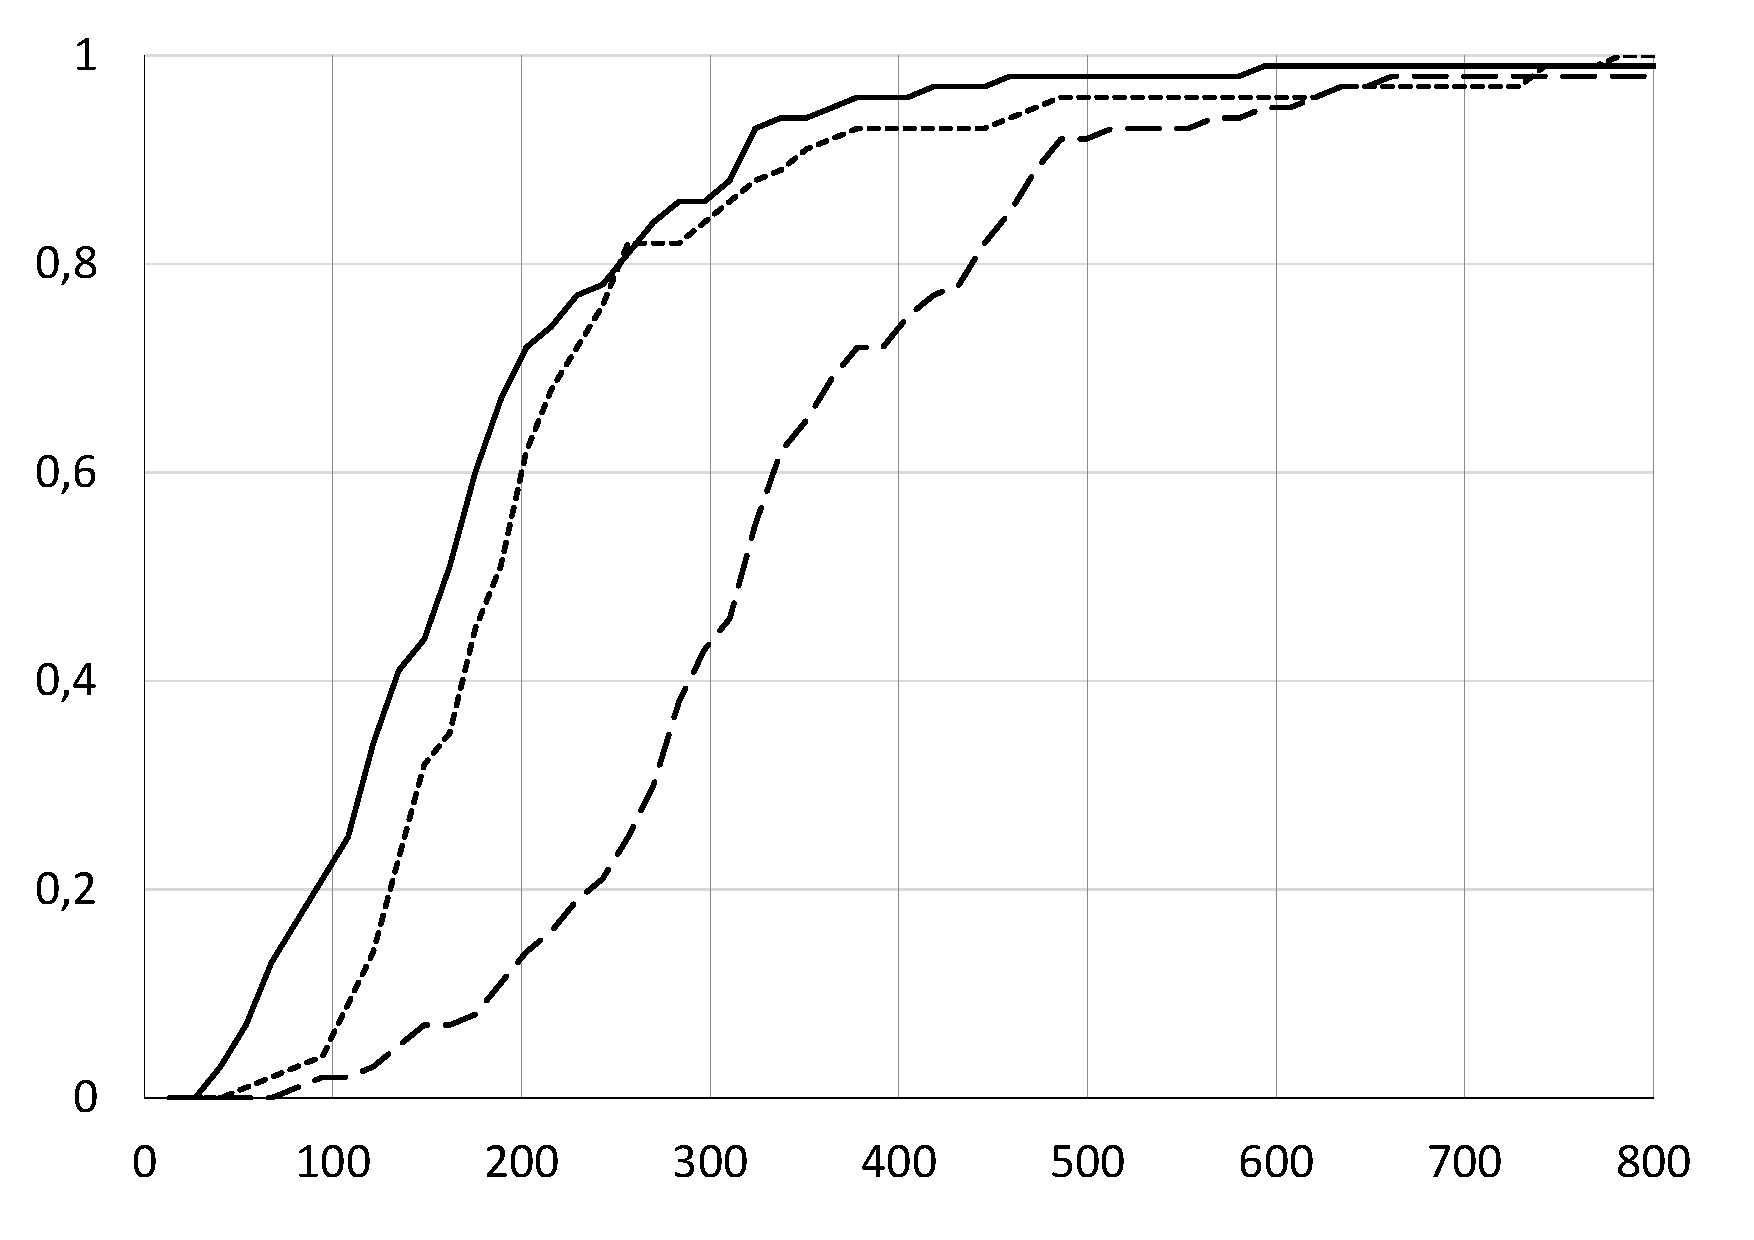
\includegraphics[width=0.50\textwidth]{2D.pdf}
\caption{Operating characteristics using $F_{gr}$ class} 
\label{fig1}
\end{figure}

\begin{figure}
\begin{minipage}{0.5\linewidth}
\center{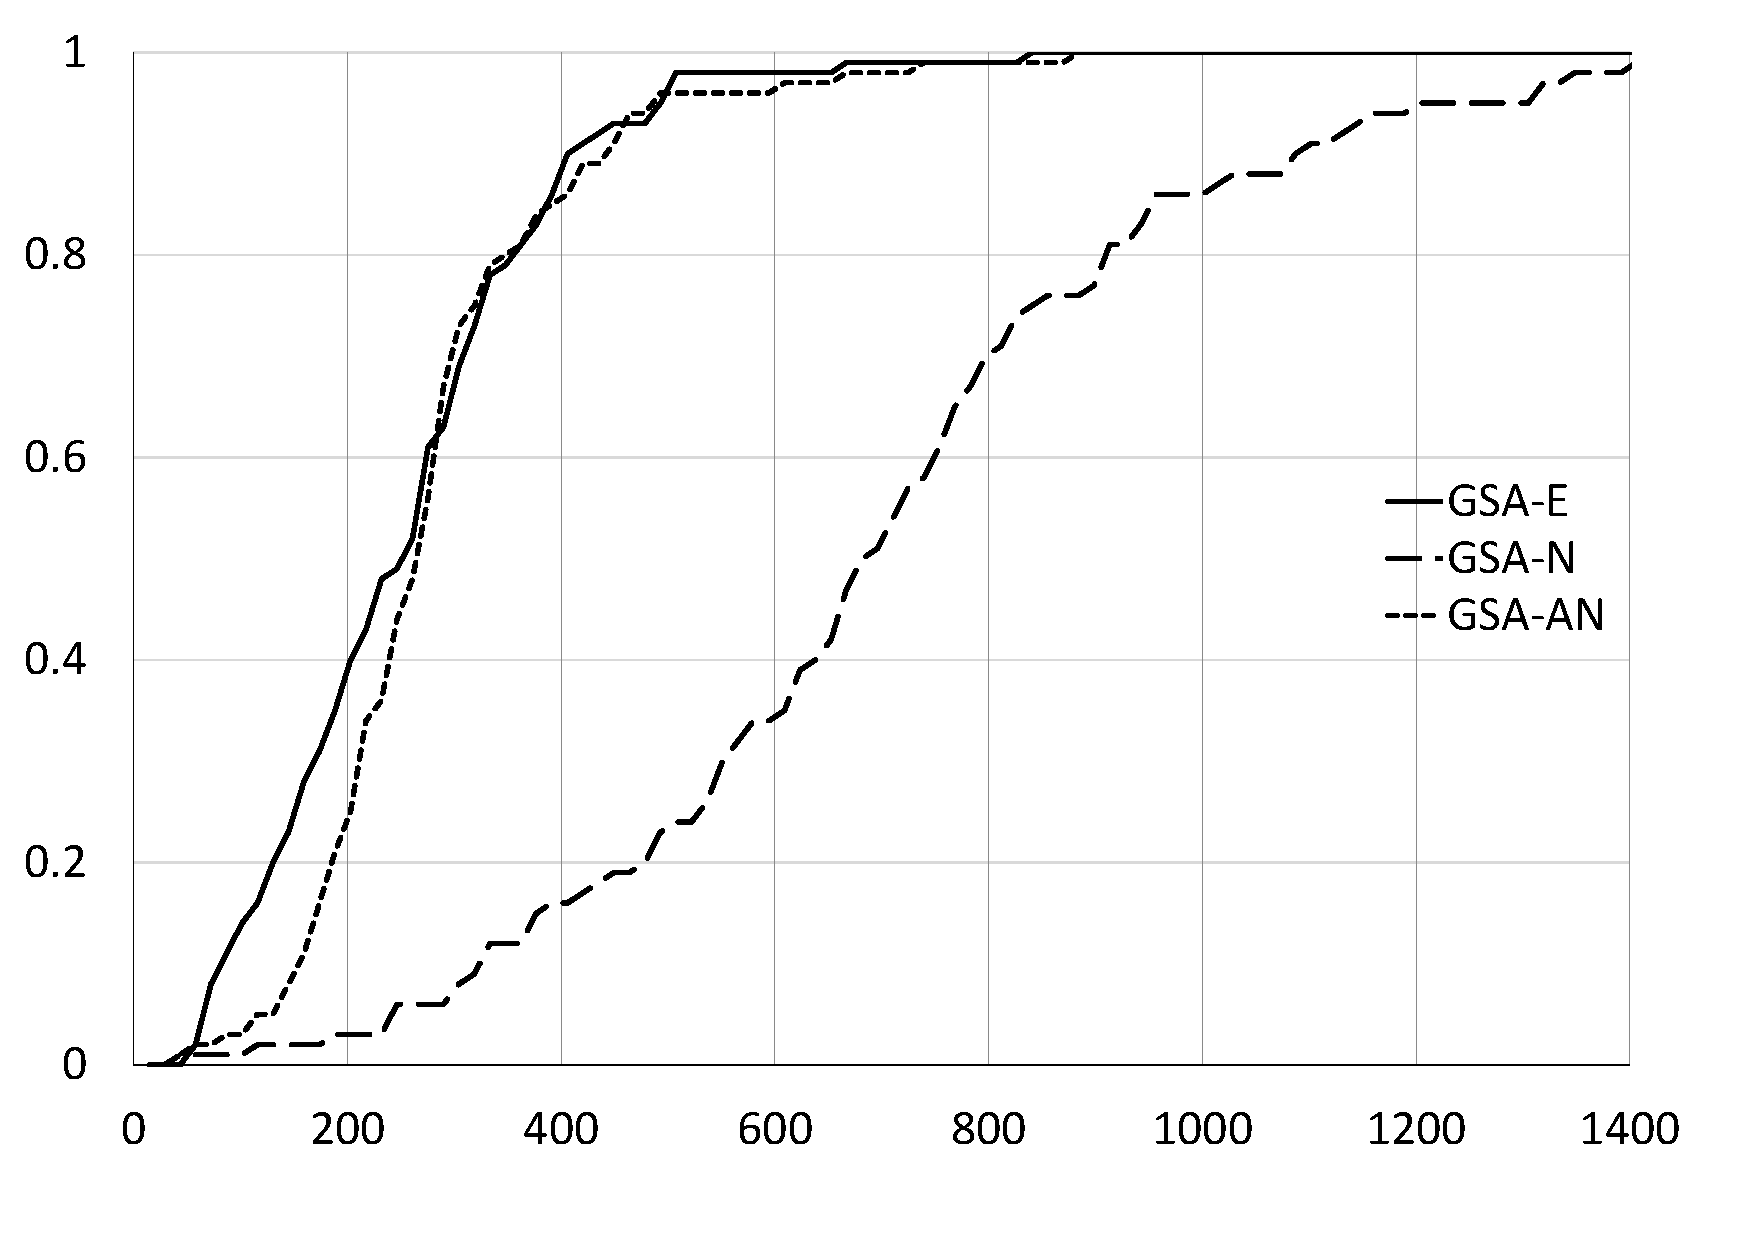
\includegraphics[width=1.0\linewidth]{2DSimple.pdf} \\ (a)}
\end{minipage}
\begin{minipage}{0.5\linewidth}
\center{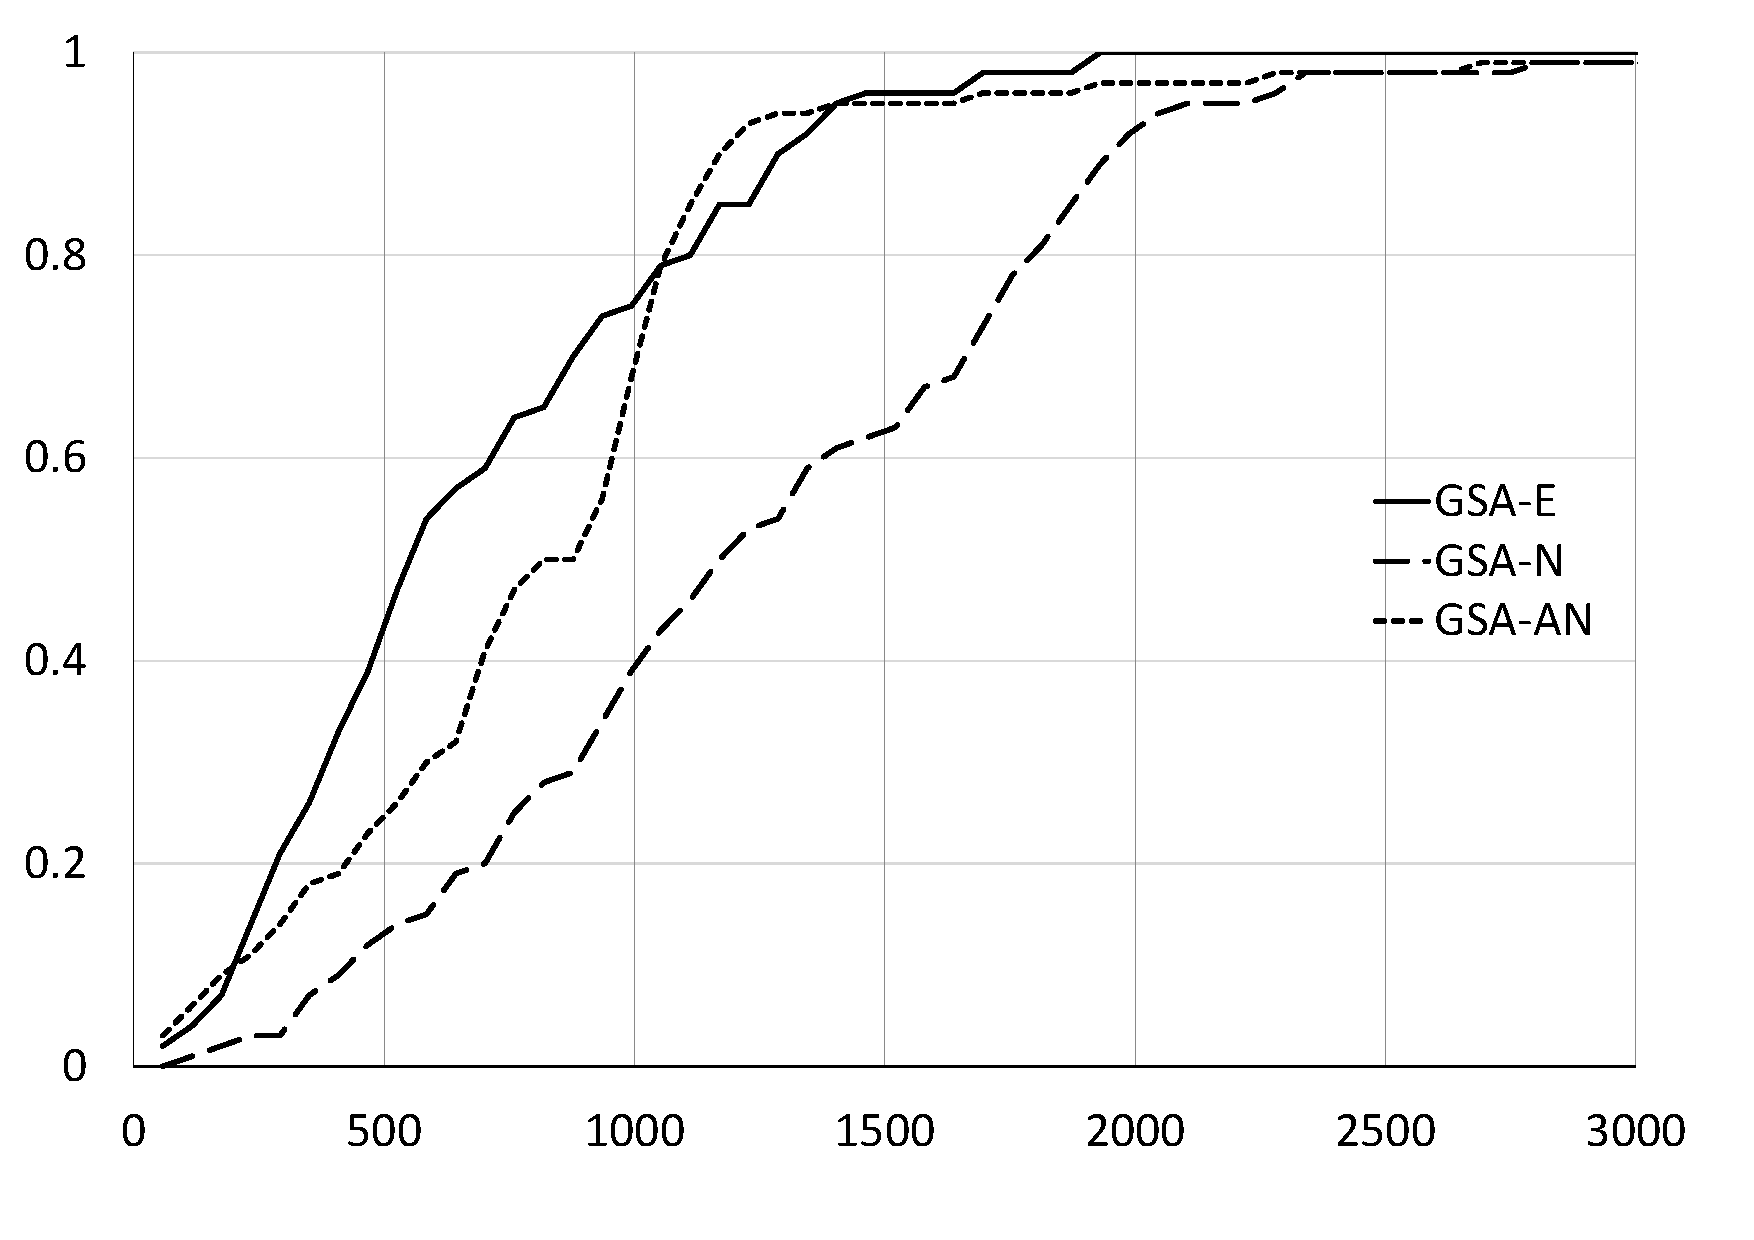
\includegraphics[width=1.0\linewidth]{2DHard.pdf} \\ (b)}
\end{minipage}
\caption{Operating characteristics using 2d GKLS \textit{Simple} (a) and \textit{Hard} (b) classes}
\label{fig2}
\end{figure}

The second series of experiments has been carried out on the four-dimensional problems from the classes GKLS 
\textit{Simple} and GKLS \textit{Hard} (100 functions of each class). Table~\ref{tab2}  presents the averaged numbers 
of trials executed by GSA with the use of the adaptive nested optimization scheme ($K_{an}$) and block adaptive nested 
optimization scheme ($K_{ban}$) with two levels of subproblems of equal dimensionality $N_1=N_2=2$. 
Note that when solving the problem of the dimensionality $N=4$ using the initial variant of the adaptive scheme, four 
levels of one-dimensional subproblems are formed that complicates the processing of these ones.

Fig.~\ref{fig3}(a,b) presents the operating characteristics of the algorithms obtained on the classes GKLS \textit{Simple} 
and GKLS \textit{Hard} respectively. The dashed line corresponds to GSA using the adaptive nested optimization 
scheme (GSA-AN), the solid line -- the block adaptive nested optimization scheme (GSA-BAN). 
The results of experiments demonstrate the use of the block adaptive nested optimization scheme provides a considerable 
gain in the number of trials (up to 35\%) as compared to the initial adaptive nested optimization scheme.

\begin{table}
\centering
\caption{Average number of trials for 4D problems.}\label{tab2}
\begin{tabular}{lcc}
\hline\noalign{\smallskip}
 &    GKLS \textit{Simple} &  GKLS \textit{Hard} \\
\noalign{\smallskip}\hline\noalign{\smallskip}
 $K_{an}$  &  21747 & 35633 \\
 $K_{ban}$ &  13894 & 31620 \\
\noalign{\smallskip}\hline
\end{tabular}
\end{table}

\begin{figure}
\begin{minipage}{0.5\linewidth}
\center{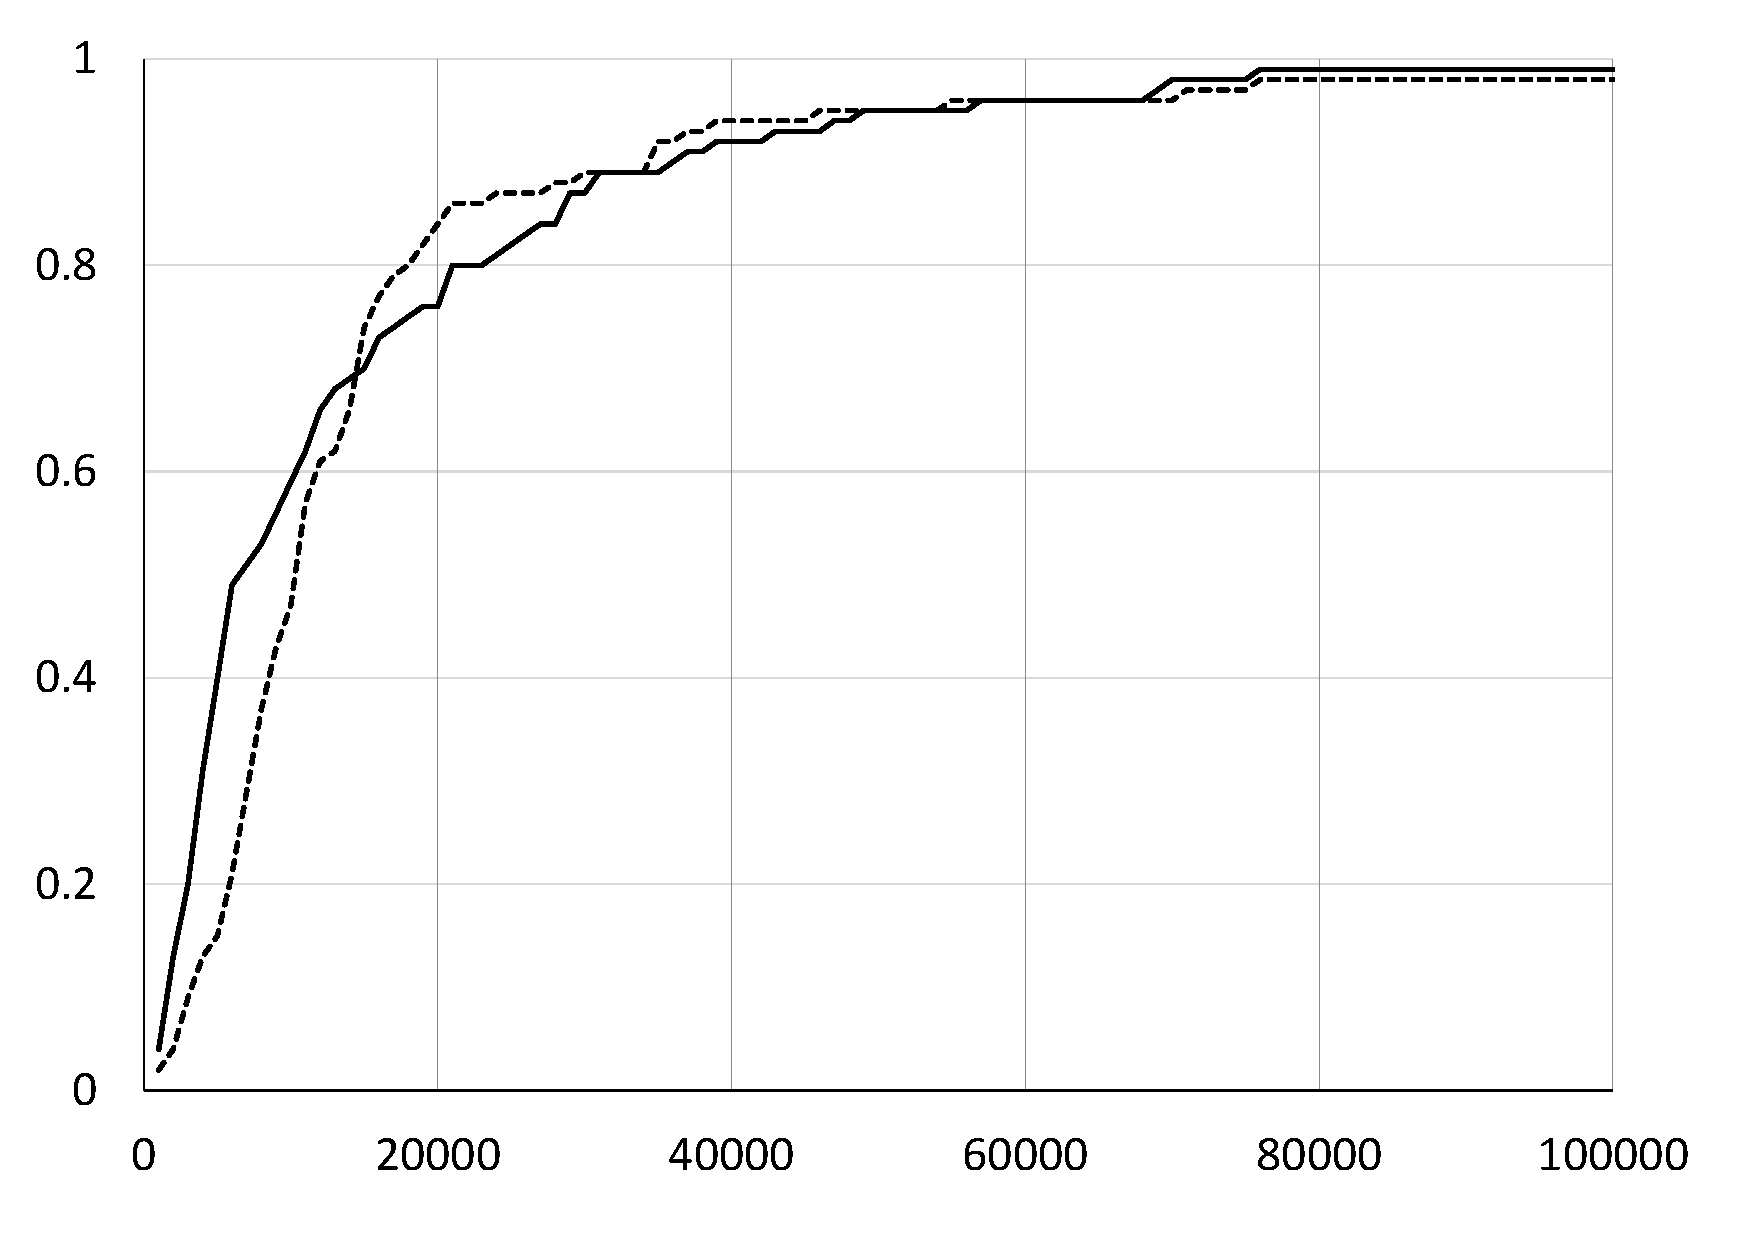
\includegraphics[width=1.0\linewidth]{4DSimple.pdf} \\ (a)}
\end{minipage}
\begin{minipage}{0.5\linewidth}
\center{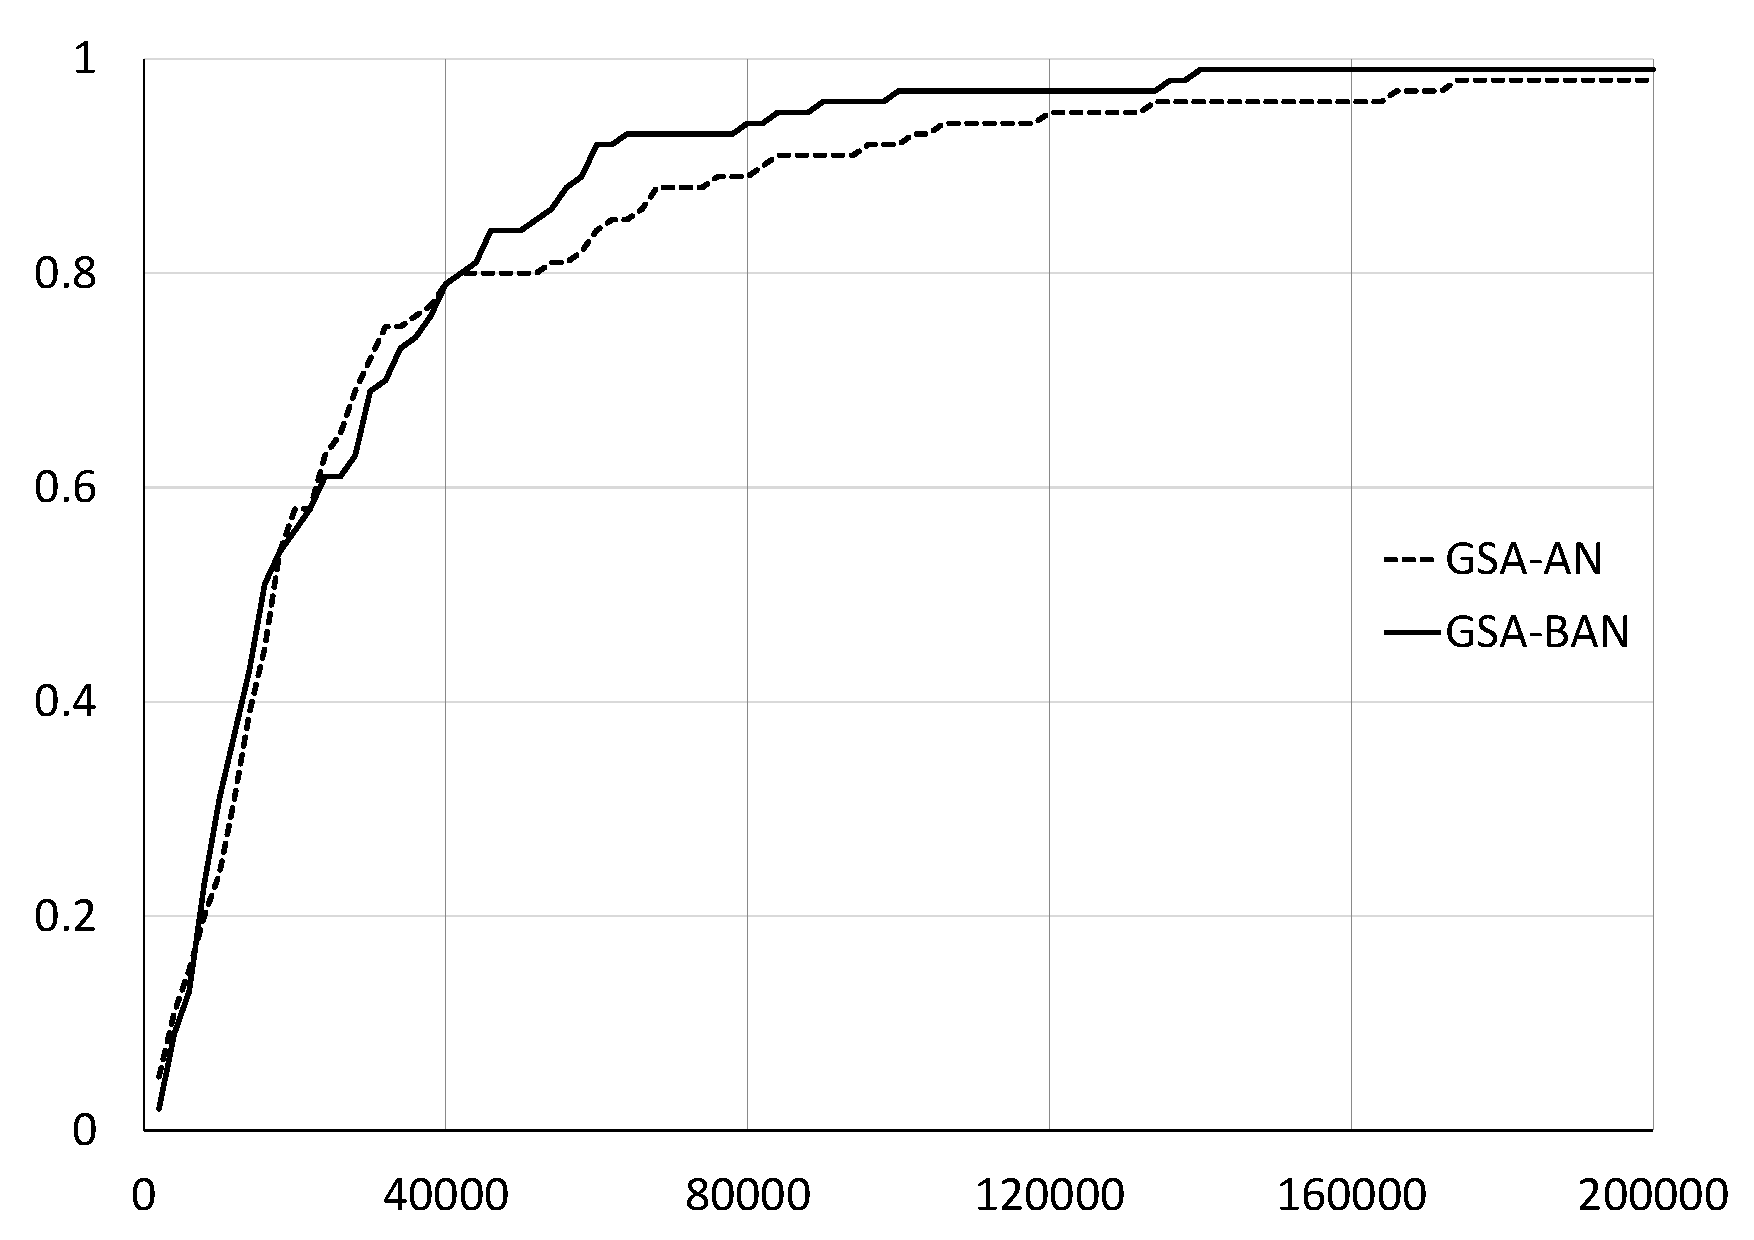
\includegraphics[width=1.0\linewidth]{4DHard.pdf} \\ (b)}
\end{minipage}
\caption{Operating characteristics using 4d GKLS \textit{Simple} (a) and \textit{Hard} (b) classes}
\label{fig3}
\end{figure}


\section{Conclusion}

In the present work, the generalized adaptive dimensionality reduction scheme for the global optimization problems 
combining the use of Peano space-filling curves and the nested (recursive) optimization scheme has been proposed.
For solving the reduced subproblems of less dimensionality, the global search algorithm was applied. 
The computational scheme of the algorithm was given, main issues related to the use of the adaptive dimensionality 
reduction scheme were considered.
The numerical experiments have been carried out using the series of test problems in order to compare the efficiencies of 
different dimensionality reduction schemes.  
The result of experiments demonstrated that the use of the block adaptive nested optimization scheme can essentially reduce the 
number of trials required to solve the problem with given accuracy. 
Further works on the development of the global optimization methods based on this method of the 
dimensionality reduction may be related to the use of the local estimates of the Lipschitz constant (considered, for example, in \cite{Grishagin2015,Sergeyev2016}) in different subproblems.


%
% ---- Bibliography ----
%
% BibTeX users should specify bibliography style 'splncs04'.
% References will then be sorted and formatted in the correct style.
%
 \bibliographystyle{splncs04}
 \bibliography{bibliography}


\end{document}
